\section{Comunicação}

Conforme explicado anteriormente, neste projeto são utilizados tanto protocolos de comunicação próprios quanto os criados por terceiros. A arquitetura desenvolvida aqui busca viabilizar a robustez do sistema, trabalhando em ambos os níveis local e remoto, com o usuário tendo o controle de sua casa por meio de um smartphone ou computador pessoal.

O serviço em nuvem recebe as requisições do usuário por meio de um cliente web ou nativo. Esse servidor processa as requisições, aplicando os filtros de segurança necessários, de modo a consultar a autenticidade do pedido e verificar se aquele usuário possui as permissões necessárias para o serviço que deseja operar. Os serviços da nuvem se comunicam com o servidor local da casa requisitada, o qual também aplica os filtros de segurança necessários e então realiza a comunicação com os módulos.

A arquitetura de comunicação é representada pela Figura \ref{fig:diagramaComunicacao} com um alto nível de abstração. Detalhes sobre a implementação e as mensagens trocadas entre servidor local, módulos e nuvem serão vistos com menor granularidade na Seção \ref{chap:morpheus}.

\begin{figure}[H]
	\centering
	\caption{Visão alto nível da comunicação no Hedwig}
	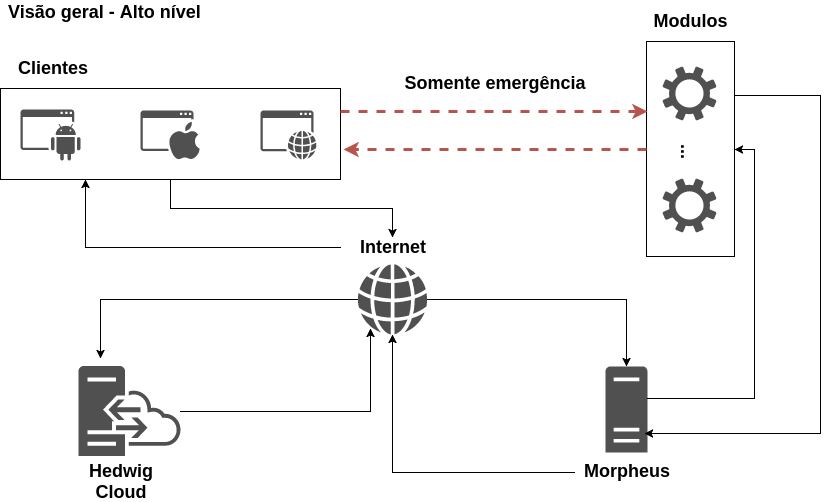
\includegraphics[width=0.8\textwidth]{arquiteturaHedwig}
	\label{fig:diagramaComunicacao}
\end{figure}

\subsection{Comunicação entre Controlador Local e Módulos}

A infraestrutura de comunicação entre o servidor local e os módulos com sensores e atuadores utiliza o protocolo de aplicação \wmqtt{}, referência em aplicações \wiot{} no mundo. O protocolo \wmqtt{} é estabelecido em cima dos protocolos TCP/IP e é orientado à sessão, diferentemente do protocolo HTTP, localizado na mesma camada \cite{ibmMqtt}.

O protocolo \wmqtt{} é do tipo \emph{Pub/Sub} (de \textit{publisher/subscriber}) e é estritamente orientado a tópicos. Assim, um \textit{subscriber} se inscreve a um tópico de seu interesse, e recebe todas as publicações que um \textit{publisher} realizar. Os tópicos são organizados com estrutura semelhante a de um sistema de arquivos Unix, com níveis hierárquicos separados por barras, de modo que o subscriber pode se inscrever para tópicos utilizando os \textit{wildcards} * e +, os quais são válidos para mais de um nível e um único nível, respectivamente \cite{mqttDocumentation}.

Para interconectar os tópicos com \textit{publishers} e \textit{subscribers}, é necessário um agente que realiza a transmissão das mensagens e que garante a segurança e confiabilidade. Esse agente é conhecido como \emph{broker} (em versões anteriores) ou \emph{server} (na versão atual, V3.1.1). O \textit{broker} permite ou nega a subscrição ou a publicação a determinado tópico. A segurança da troca de mensagens é realizada por meio do protocolo TLS (\textit{Transport Layer Security}) que encripta os segmentos na camada de transporte.

O protocolo \wmqtt{} também oferece três tipos de QoS (\textit{Quality of Service}), possibilitando: diminuir o \emph{overhead} ao máximo, enviando a mensagem uma única vez, na configuração mais simples; garantir que a mensagem seja entregue no mínimo uma vez, na configuração de segundo nível; garantir que a mensagem seja entregue exatamente uma vez, no terceiro nível, o que consequentemente aumenta o \emph{overhead}.

As mensagens são transmitidas em texto puro, e é necessário estabelecer um protocolo para a sua utilização. Foi desenvolvido um protocolo de fácil utilização e com baixo \emph{overhead}, mas que pudesse ser expansível e flexível aos casos de uso desejados.

O \textit{broker} Mosquitto\footnote{https://mosquitto.org/} é utilizado no Hedwig. Ele foi escolhido por ser amplamente adotado em projetos de \wiot{}, além de ser \emph{open-source} e ter licença abrangente (MIT). Entretanto, há outras diversas possibilidades, como o HiveMQ, adotado no projeto HomeSky e com grande uso em aplicações enterprise \cite{hiveMq}.

\subsection{Comunicação entre Controlador Local e Nuvem}

Inicialmente, foi proposto um modelo arquitetural para a comunicação com a nuvem no qual existiriam \emph{endpoints} para requisições HTTP tanto do lado da casa quanto do lado da nuvem. Assim, quando o Morpheus precisasse enviar uma mensagem, seria necessário realizar uma chamada ao \emph{endpoint} correspondente. Neste sentido (Morpheus para nuvem) não há nenhum problema, pois é possível garantir as configurações avançadas de segurança adequadas, bem como a utilização de balanceadores de carga e servidores terceiros para lidar com ataques do tipo DoS \cite{akamai}, conforme RNF-6.

O problema, no entanto, está em garantir a segurança e usabilidade do lado da casa. Primeiramente, os IPs residenciais não são fixos, sendo trocados a cada nova conexão. Assim, se a conexão com a Internet for perdida, por exemplo, um novo IP será atribuído àquela residência. Dessa forma, após essa troca, a não ser que o Morpheus atualize a nuvem, não seria possível receber as mensagens que chegariam dos serviços remotos. Esta questão, no entanto, é contornável por meio de um serviço de \emph{watchdog}, que seria responsável por analisar o IP e notificar a nuvem sobre a troca sempre que esta ocorrer. Há, ainda, um problema mais grave e mais difícil de ser contornado. Com essa arquitetura, o Morpheus também seria um servidor do ponto de vista da nuvem, e qualquer dispositivo poderia tentar fazer uma requisição em um dos \emph{endpoints} disponíveis. Mesmo que sejam checados os dados da requisição para garantir que ela seja válida, tem-se ainda uma grave ameaça de segurança em relação à negação de serviço. Para que este risco fosse minimizado, seriam necessárias configurações avançadas no roteador local, e, mesmo assim, este não seria suficiente para processar um grande número de requisições, deixando a casa vulnerável.

Uma forma de contornar o problema se encontra no uso de WebSockets, protocolo detalhado na Seção \ref{sub:websocket}. Assim, o Morpheus se comporta como um cliente em relação à nuvem e é sempre ele que abre uma conexão. Essa conexão se mantém aberta e forma um caminho \emph{full-duplex}, de modo que é possível receber as mensagens da nuvem a qualquer momento também. Com essa arquitetura, os desafios relativos à segurança recaem aos servidores e não mais à casa, de modo que é possível gerenciar esses riscos como o fazem grandes empresas, ou seja, de forma transparente ao cliente final.

\subsection{Comunicação entre Nuvem e Aplicativos}

Similarmente à comunicação entre controlador local e nuvem, a troca de informações entre nuvem e aplicativos clientes em geral é feita por meio de WebSockets. Como aplicações web podem ter como requisito oferecer suporte à navegadores mais antigos, é usado um \emph{fallback} para um mecanismo de \emph{polling} caso não haja suporte para WebSockets.

\subsection{Comunicação entre Módulos e Aplicativos}

Em caso de indisponibilidade da rede local ou internet, a comunicação é feita diretamente entre módulos e aplicativo backup com escopo local (por meio de HTTP). Esse canal de comunicação fica aberto para uso somente nesses casos, para evitar exposição desnecessária a possíveis ataques. O módulo atua como servidor e o aplicativo como cliente, sendo que cada aplicativo pode se conectar diretamente ao módulo que desejar.

\subsection{Diagramas de Sequência}

Seguem diagramas de sequência UML para ilustrar a comunicação fim a fim utilizada no projeto:

\begin{figure}[H]
	\centering
	\caption{Diagrama de Sequência - Data Transmission}
	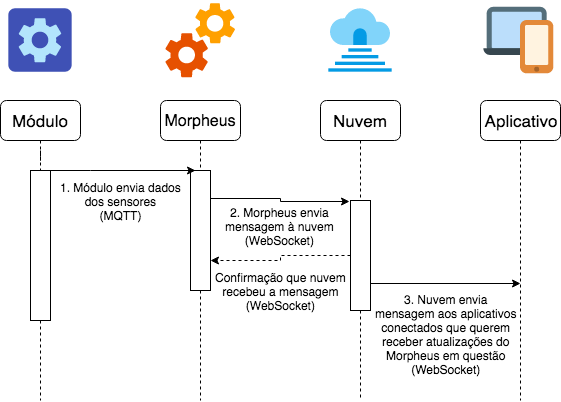
\includegraphics[width=1\textwidth]{sequencia_data}
	\label{fig:sequencia_data}
\end{figure}

No sistema instalado nas residências para coleta de dados, ocorre atualização a cada 1 minuto. No caso de mudança considerável no estado de algum sensor ou acionamento de algum relé, há uma atualização para o aplicativo com tempo de resposta de 1 segundo.

Para os casos de mudança de configuração e atuação (acionamento de relés), temos:

\begin{figure}[H]
	\centering
	\caption{Diagrama de Sequência - Configuration e Action Request}
	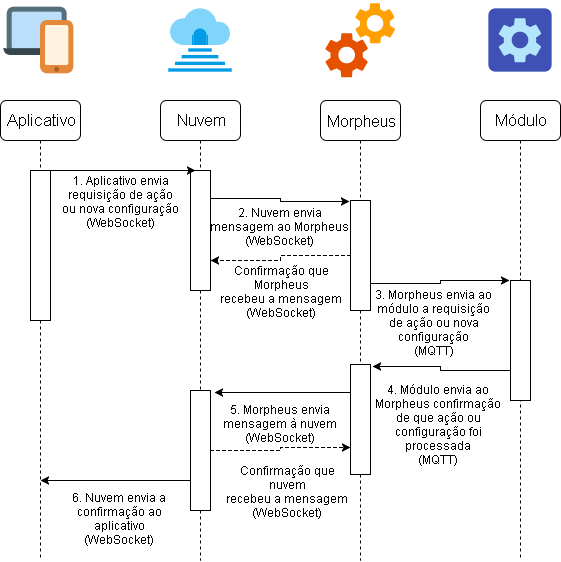
\includegraphics[width=1\textwidth]{sequencia_action_configuration}
	\label{fig:sequencia_action_configuration}
\end{figure}

Se não houver conexões disponíveis, os procedimentos de atualização de estado de dados, requisição de ação e configuração ocorrem diretamente entre módulos e aplicativos. O usuário ainda pode atuar no sistema através de controles de rádio frequência e botões físicos, utilizando uma comunicação direta entre usuário e módulo (sem uso do aplicativo).

\begin{figure}[H]
	\centering
	\caption{Diagrama de Sequência - Data Transmission do Aplicativo Backup}
	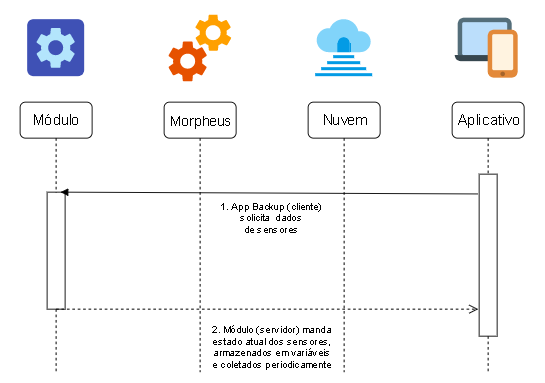
\includegraphics[width=1\textwidth]{app_backup-sequencia_data}
	\label{fig:app_backup-sequencia_data}
\end{figure}

\begin{figure}[H]
	\centering
	\caption{Diagrama de Sequência - Configuration e Action Request do Aplicativo Backup}
	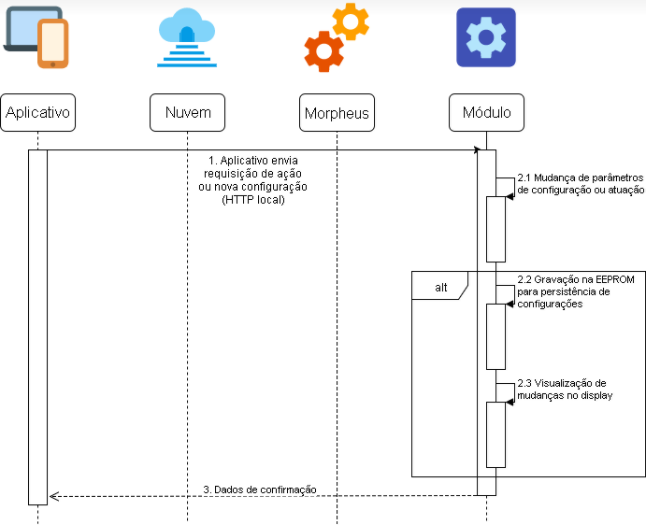
\includegraphics[width=1\textwidth]{app_backup-sequencia_action_configuration}
	\label{fig:app_backup-sequencia_action_configuration}
\end{figure}

É importante destacar que não há possibilidade do usuário requisitar múltiplos acionamentos (causando muitas trocas de estado em um período pequeno de tempo), uma vez que a requisição é realizada a partir do estado atual do relé (dessa forma, se este estiver ativo, múltiplos cliques do usuário mandam a requisição ``desligar'').

Outro ponto é a inclusão de um mecanismo simples para segurança do sistema, mesmo no canal de comunicação emergencial de escopo local, mostrando uma possibilidade de aumento do nível de segurança do sistema (maiores detalhes estão na seção \label{acessomodulo}).

\begin{figure}[H]
	\centering
	\caption{Diagrama de Sequência - Action Request com Senha no Aplicativo Backup}
	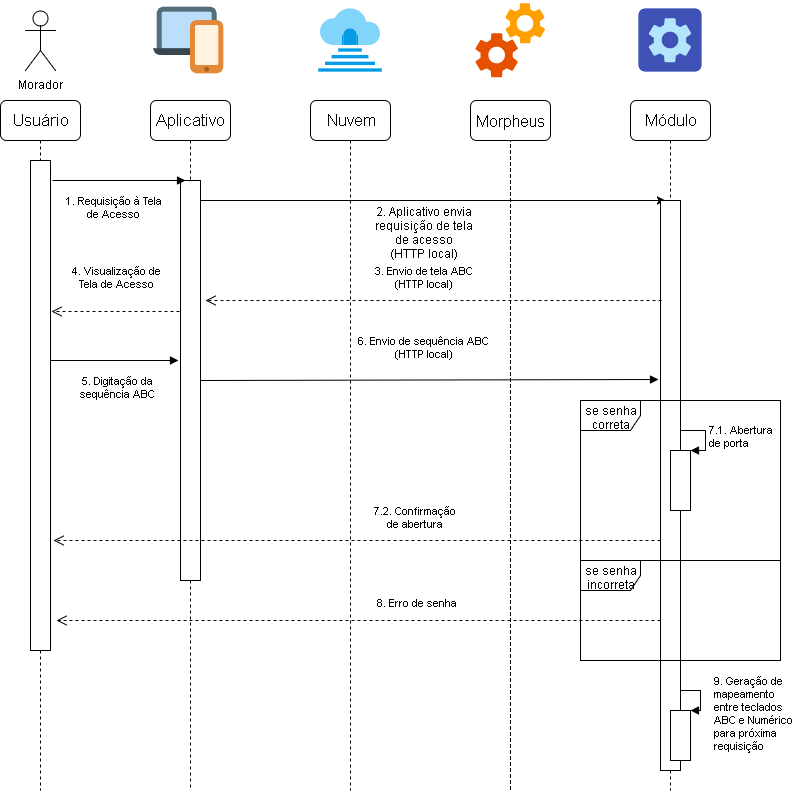
\includegraphics[width=1\textwidth]{app_backup-sequencia_action_seg}
	\label{fig:app_backup-sequencia_action_seg}
\end{figure}
